\chapter{Projektplanung}\label{ref:projektPlanung}
Die Projektidee entstammt von studentischer Seite. In Abbildung
\ref{ref:wolkeMM} ist daher eine Wortwolke zu sehen, in der in Stichworten
beschrieben ist, was sich unter Masterly Mate vorzustellen ist.

\begin{figure}[H]
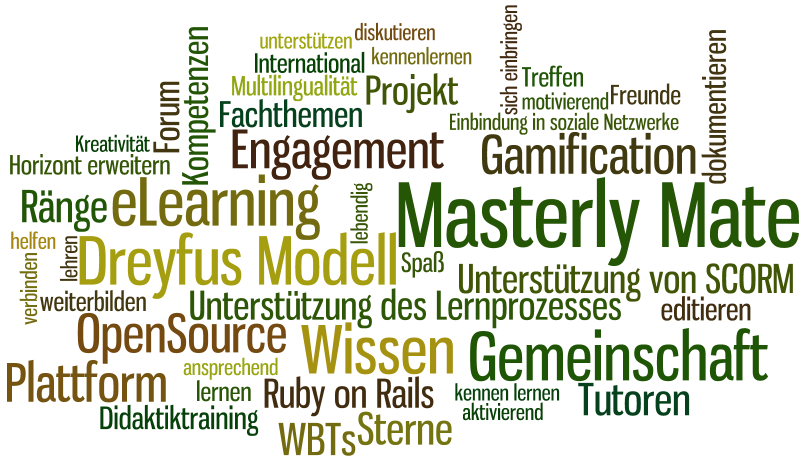
\includegraphics[width=1\textwidth]{MasterlyMateWolke.png}
\caption{Wortwolke beschreibender Begriffe der "`Masterly
Mate"'-Idee}\label{ref:wolkeMM}
\end{figure}

Das Projekt nimmt sich eine Art Lernplattform zum Ziel, auf der Lernende auf
Lehrende treffen sollen. Dabei entstehen Situationen, in der eine lehrende
Person zu einer lernenden wird, und umgekehrt. Es sollen Diskussionen über
bestimmte Fachgebiete stattfinden können und ideale Tutoren für bestimmte
Fragestellungen gefunden werden. Da es nichts zu gewinnen gibt, engagiert sich
jeder Teilnehmer freiwillig. Er erhält Wissen und kann dieses im nächsten Moment
an weitere interessierte Personen weitergeben, was sein eigenes Wissen erneut
festigt. Lehrstunden sollen im gemütlichen Umfeld, wie Caffees oder Parks
stattfinden. Dem Duo steht es auch offen auf andere Kommunikationskanäle, wie
Chat oder E-Mail, zu wechseln. Jeder Nutzer kann als Tutor für sein Fachgebiet
oder seine Fachgebiete fungieren.

Um stets einen idealen Tutor zu finden, folgt die Idee dem Dreyfus fünf Etappen
Modell mentaler Aktivitäten, welches in Abschnitt \ref{ref:dreyfus} näher
beschrieben wird. So ist gewährleistet, dass ein Neuling die Inhalte von einer
Person erklärt bekommt, die selbst noch im Lernprozess steckt und es können
Inhalte, Tipps und Hinweise auf passendem Niveau ausgetauscht werden.

Letztlich soll das Ziel der Mitgliedschaft auf der Plattform nicht sein, der
beste Guru eines Faches oder der beste Lehrer zu werden. Es geht darum
Teil einer Bildungsgemeinschaft zu sein und sich gegenseitig engagiert zu
unterstützen.

\section{Motivation und Notwendigkeit}\label{ref:projectMotivation}
Die Motivation zu dieser Idee entstand aus der interessanten und
erwartungsvollen Kombination von eLearning\footnote{siehe Abschnitt
\ref{ref:basELearning}} und Gamification \footnote{siehe Abschnitt
\ref{ref:gamification}}. Hinzu kommt die heute populäre Vorstellung von Blended
Learning \footnote{siehe Abschnitt \ref{ref:blendedLearning}}, wodurch das doch
sehr trockene und eintönige Durcharbeiten von WBTs\footnote{siehe Abschnitt
\ref{ref:basWBT}} durch Lehreinheiten mit einem Tutor unterstützt wird.

Masterly Mate soll eine zentrale Anlaufstelle für diverse Weiterbildungs- und
Lernangelegenheiten sein. Unabhängig davon, ob die Motivation privatem Interesse
oder dem eigenen Bildungsweg entspringt, soll jeder Interessent wissen, dass
die Plattform Antworten bietet.

Die Notwendigkeit resultiert aus der fehlenden Fähigkeit des Internets,
Sachverhalte erläutern zu können. Heute ist es Usus beim Recherchieren das
Internet zu gebrauchen, in dem rohe Daten und Informationen vorliegen. Wissen
ist dort eher rar. Es gibt bisher nur wenige Plattformen, wie Wikipedia, die
existieren, um Wissen zu publizieren, jedoch fehlt auch dort eine erklärende und
erläuternde Komponente durch einen Menschen. Dieses Manko soll Masterly Mate
ausgleichen.

\section{Abgrenzung}
Das Projektergebnis behauptet keinen Anspruch auf ein vollwertiges \ac{LMS}. Es
fehlt die Komponente zur Organisation kompletter Lernpakete. In Masterly Mate
stehen die WBTs unabhängig da. Sie sind allein Mittel zum Zweck als Beleg für
die fachliche Kompetenz.

Weiterhin soll es Wikipedia nicht ersetzen. Das Projektergebnis bietet keine
ausformulierten Texte oder Artikel zu Lerninhalten. Der Fokus liegt wesentlich
stärker auf der Komponente Wissen zu vermitteln.

\section{Zielsetzung}
Da das Projekt insgesamt auf einen längeren Zeitraum angesetzt ist, lässt es
sich nicht innerhalb der Bearbeitungszeit der vorliegenden Studienarbeit
umsetzen. Aus diesem Grund sind die Ziele zum einen in operative und zum anderen
in strategische zu unterteilen. 

\subsection{Operative Ziele}
Wie in Kapitel \ref{ref:chaptIntroduction} bereits angerissen wurde, soll zu
Projektende ein funktionaler Prototyp stehen. Auch ist ein Konzept angedacht,
welches der einfachen Weiterentwicklung und Verbreitung von Masterly Mate dient.
Eventuell wird sich bis dahin eine kleine, lebendige Gemeinschaft gebildet
haben, die die Plattform nutzt und um Inhalte erweitert. Die ersten Nutzer
sollen automatisch unabhängig ihres didaktischen Grades\footnote{näher erläutert
in Abschnitt \ref{ref:rankTeach}} Autoren sein. So ist gewährleistet, dass
Inhalte für neue Nutzer bereits existieren.

Das Projekt als Ganzes soll einen leichten Start haben. Sind die Ziele für die
ersten Nutzer zu hoch gesteckt, resultiert aus der geringen Anzahl von Anwendern
und den damit schwer erreichbaren nächsten Rängen Frustration und Unwille zur
Nutzung der Plattform. Somit ist angedacht, die erforderliche Punktzahl für
höhere Ränge (siehe Abschnitt \ref{ref:dreyfus}) mit der Anzahl an Benutzern zu
skalieren.

\subsection{Strategische Ziele}
Längerfristig betrachtet soll eine rege und große Gemeinschaft entstehen, die
Hilfsbereitschaft nicht scheut. Dazu wird bereits zu Beginn der Entwicklung eine
Internationalisierung\footnote{siehe Abschnitt \ref{ref:internationalisierung}}
berücksichtigt. Masterly Mate soll zur, in Abschnitt \ref{ref:projectMotivation}
beschriebenen, zentralen Anlaufstelle heranwachsen.

Dabei werden, um den Reiz am Lernen zu erhöhen, mit der Menge der Nutzer die
Anforderungen für die jeweils nächsten Ränge erhöht. Denn je mehr Beteiligung
die Plattform erfährt, desto wahrscheinlicher ist es, einen Tutor in der
jeweiligen Region zu finden. Damit wird es auch immer einfacher, Punkte für den
didaktischen Rang zu sammeln.

Weitere akute, sowie optionale Vorhaben sind in Kapitel \ref{ref:chaptSummary}
am Ende des vorliegenden Dokuments nach der tatsächlichen
Implementierung aufgeführt.
